\documentclass{sig-alternate-05-2015}
\makeatletter
\def\@copyrightspace{\relax}
\makeatother

\usepackage[ruled]{algorithm2e}
\usepackage{amssymb}
\usepackage{algorithmic}
\usepackage{listings}
\usepackage{stmaryrd}
\usepackage{graphicx}
\usepackage{color}
\usepackage{comment}
\usepackage{url}

\widowpenalty=10000
\clubpenalty=10000

\pdfpagewidth=8.5in
\pdfpageheight=11in

\begin{document}

% Copyright
\setcopyright{acmcopyright}
%\setcopyright{acmlicensed}
%\setcopyright{rightsretained}
%\setcopyright{usgov}
%\setcopyright{usgovmixed}
%\setcopyright{cagov}
%\setcopyright{cagovmixed}
\doi{10.475/123_4}

\isbn{123-4567-24-567/08/06}
\conferenceinfo{PLDI '13}{June 16--19, 2013, Seattle, WA, USA}
\acmPrice{\$15.00}
\conferenceinfo{WOODSTOCK}{'97 El Paso, Texas USA}

\title{PCC: Practical Code Completion Tool with Fuzzy Matching and Precise Synthesis on Statistical Language Modelling}\vspace{-2cm}

\numberofauthors{1}
\author{
\alignauthor
Yixiao Yang \\
       \affaddr{Tsinghua University, TNLIST, KLISS, Beijing, China} \\
       \email{yangyixiaofirst@163.com}
}
\date{15 July 2016}
\maketitle
\begin{abstract}
% In fact, many people write the already written code.
As open source has become a trend, more and more good projects can be found on github. In countless projects, much of the code can be similar. But in most cases, the existing code cannot be directly copied and pasted. Besides, searching for similar code is difficult, especially for structurally similar one.

% Usually, people prefer to write code directly, instead of spending much time to search the similar code to modify it.

We present PCC\footnote{Hhhaha}, a plugin of eclipse IDE which analyzes the code being written, uses the sequence fuzzy matching algorithm to find similar contexts, predicts the most likely sequence based on the pre-trained statistical language model and automatically synthesizes the code from the sequence.

PCC is an intelligent code writer which synthesizes a whole statement which may include all syntax elements of Java in real time. PCC takes the context of currently being edited Java file into consideration and ensures that there are no compilation errors in the generated code.

The correctness of the completed code is 95\% among 100 test cases. The time cost of 80\% of the completion process is less than 2 seconds, which is effective and user-friendly. In the worst case, the time cost is still less than 4 seconds. To best of our knowledge, it is the first time to apply fuzzy matching algorithm to match and predict the code patterns on the statistical language model. It is also the first time to make a practical tool to automatically write the code with no compilation errors.
\end{abstract}

\begin{CCSXML}
<ccs2012>
<concept>
<concept_id>10011007.10011074.10011784</concept_id>
<concept_desc>Software and its engineering~Search-based software engineering</concept_desc>
<concept_significance>500</concept_significance>
</concept>
</ccs2012>
\end{CCSXML}
\ccsdesc[500]{Software and its engineering~Search-based software engineering}
\printccsdesc

\vspace{-0.1cm}
\keywords{Code Completion, Code Prediction, Synthesis, Automatically Code Writing, Statistical Language Modelling}

\section{Introduction}

Since 2012, researchers have tried to apply different machine learning algorithms to software engineering. When applying algorithms of natural languages to source codes, things become more complicated. Unlike natural languages, source codes are closely related. Minor modifications may cause compilation errors. This brings challenges to automatic code generations.

PCC synthesizes codes based on patterns which is different from Test Driven Synthesis technique which is based on genetic algorithms. There have been multiple code synthesis and auto-fix tools \cite{DBLP:conf/icse/WeimerNGF09}\cite{nguyen2013semfix}\cite{perelman2014test} driven by genetic algorithms. These tools can generate accurate code based on oracle test cases. However, there is still a long way to achieve the goal of automatic code writing. Although the integer expression synthesis and the Boolean expression synthesis have been developed for a long time, the problem synthesizing with external method invocations is still difficult. There would be too many possible situations. The genetic algorithm is slow for the problem of a large size.

To narrow the whole possible search space, applying machine learning algorithms to big-code to learn how to write codes has become an effective method.

We apply n-gram model to train the source codes of Java. We predict the codes which are of highest probabilities based on the trained n-gram model.

%Because the improvements brought by different n-gram algorithms are small, PCC uses the basic n-gram model.
%and the fuzzy matching with precise synthesis is the vital concern,

%Given a sequence of tokens, the last n-1 tokens are used as the longest context to infer the next token with the n-gram model. The tokens with the highest conditional probabilities will be inferred.

\vspace{-0.2cm}
\section{Related Work}

The first one to apply natural language processing algorithms to source codes was Hindle \cite{DBLP:conf/icse/HindleBSGD12}, he used the n-gram \cite{cavnar1994n} model to train the source codes of Java. The next work was done by Allamanis \cite{DBLP:conf/msr/AllamanisS13a}, he trained 100 times larger model than Hindle and made a topic visualization tool to show the frequently used codes of the software. Nguyen \cite{DBLP:conf/sigsoft/NguyenNNN13} refined the tokens, used the n-gram topic \cite{wang2007topical} model, performed the experiments similarly. Nguyen \cite{DBLP:conf/icse/NguyenN15}, Raychev and Vechev \cite{DBLP:conf/pldi/RaychevVY14} used the statistical language model to do the theoretical research on API usages.

The previous works can hardly predict and synthesize the codes which can actually be used. The reason is that their models are too scattered.

For example, ``String str=a.toString()'' will be split into 8 tokens: String$\#$str$\#$=$\#$a$\#$.$\#$toString$\#$($\#$). Every word split by $\#$ is a token. If a 5-gram model is available, when inferring the next token from the above example, what will be inferred? Now the longest context is the last 4 tokens: .\#toString\#(\#). Even with the longest context, any token behind statements such as ``String str=a.toString()'', ``String any=anything.toString()'', ``print(sth.toString())'' and so on will show up. Information before ``.toString()'' is lost. According to our experiments, if the model is large, about 100 different tokens with similar probabilities will be obtained. Choosing the next token has become a problem. What is more, different people have their own name conventions. Some people like to declare variable like this: ``String ssssss1 = a.toString()''.

The model cannot be compact either. Due to the database being searched by the exact key, if taking the statement ``String str=a.toString()'' as one token, nothing will be inferred from the statement ``String str=b.toString()'' although there is only one character different between two tokens.

Therefore, we propose a novel code completion tool. An intermediate representation of Java codes is introduced and the fuzzy matching algorithm is used.

\section{Architecture}

Figure \ref{architecture} shows the architecture and the execution flow of PCC.
\vspace{-0.25cm}
\\\begin{figure}[htbp]
  \centering
  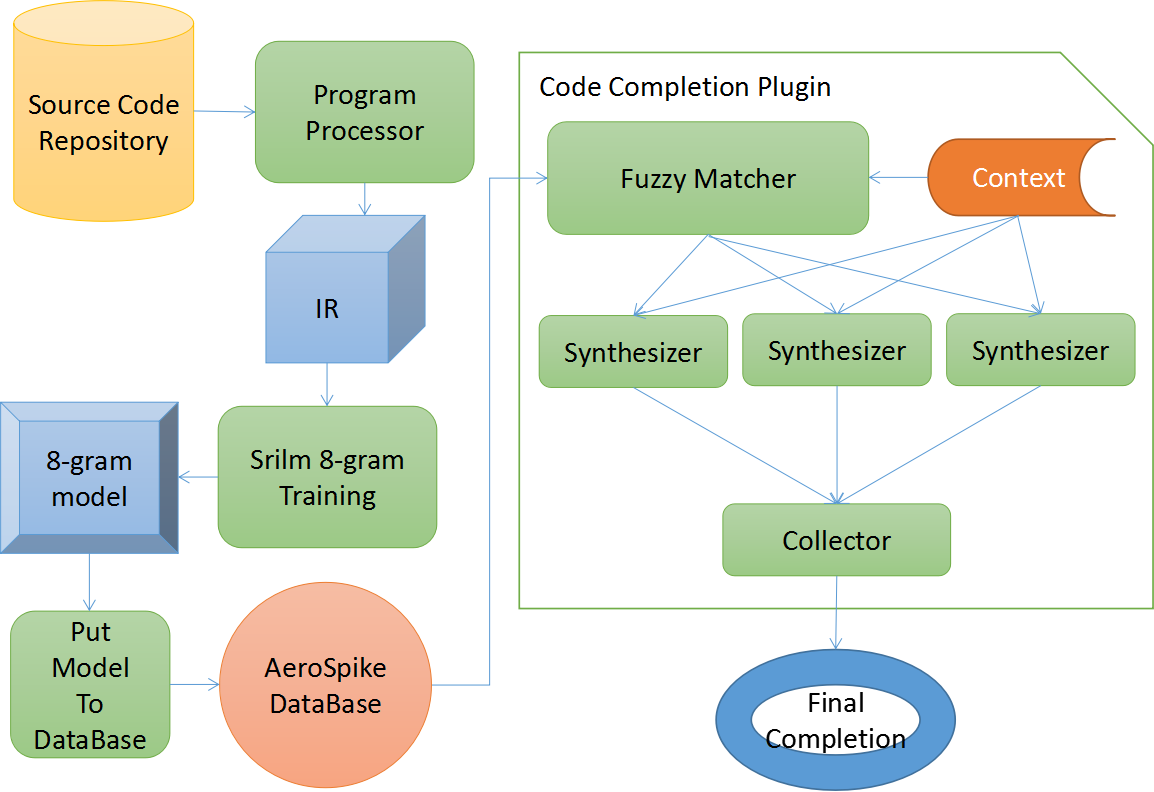
\includegraphics[width=0.48\textwidth]{pics/architecture.png}\\
  \caption{PCC architecture}\label{architecture}
\end{figure}

Source Code Repository contains Java source files crawled from github and other websites. Program Processor translates Java source files to IR. IR is a special form which meets the condition: one operation one token. The basic idea is that if a statement is too long, we split it into several tokens. IR is carefully designed to ensure that these separated tokens can be rebuilt to the original statement. Variable names are eliminated in IR. Due to one token contains only one operation, it is easy for IR to do sequence fuzzy matching. As discussed in Related Work, IR cannot be too scattered nor too compact. After trying for 2 months, a suitable kind of IR was finally found.
\vspace{-0.25cm}
\\\begin{figure}[htbp]
  \centering
  % Requires \usepackage{graphicx}
  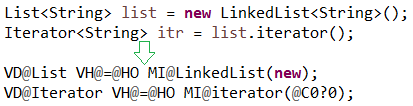
\includegraphics[width=0.3\textwidth]{pics/toIR1.png}\\
  \vspace{-0.15cm}
  \caption{Simple translation to IR}\label{toIR1}
\end{figure}

Firgure \ref{toIR1} gives a concrete idea about the translation and the IR. VD@ means a type declared. VH@ means a variable declared.
@HO means that some operations are after this token. MI@ means the method invocation.

Notice that, In Figure \ref{toIR1}, the strange symbol $C0?0$ refer to the variable ``list'' which is of type $List<String>$.

Figure \ref{vartoIR1} shows the translation rule of the variable name.

Figure \ref{moretoIR} shows more examples about the IR translation.

%In IR, every word split by white spaces or line breaks is a token. So there are three tokens in the following line:
%VD@List\quad\ \  VH@=@HO\quad\ \  MI@LinkedList(new);

The grammar of the IR is available in \cite{irgrammar}. The program which can parse the IR is available in \cite{irparser}.

Then the IR is trained by Srilm\cite{stolcke2011srilm} tool. If the Srilm[10]
tool is told to train 3-gram models, the 2-gram model and 1-gram model will also be trained. So, if the 8-gram model is trained, the 1-gram to 7-gram models are also be trained.
\vspace{-0.4cm}
\\\begin{figure}[htbp]
  \centering
  % Requires \usepackage{graphicx}
  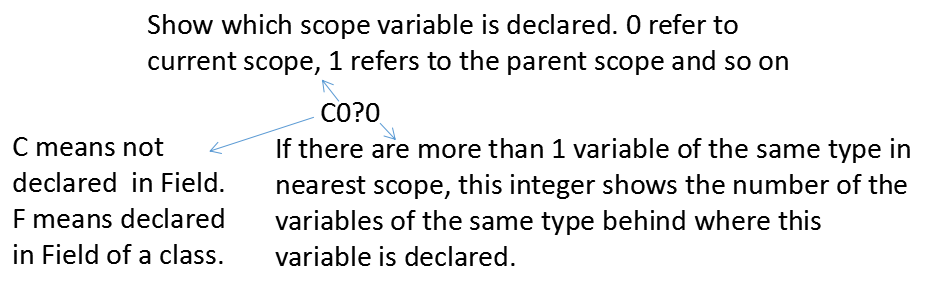
\includegraphics[width=0.4\textwidth]{pics/variableIR.png}\\
  \vspace{-0.1cm}
  \caption{Variables to IR}\label{vartoIR1}
\end{figure}
\vspace{-0.4cm}
\\\begin{figure}[htbp]
  \centering
  % Requires \usepackage{graphicx}
  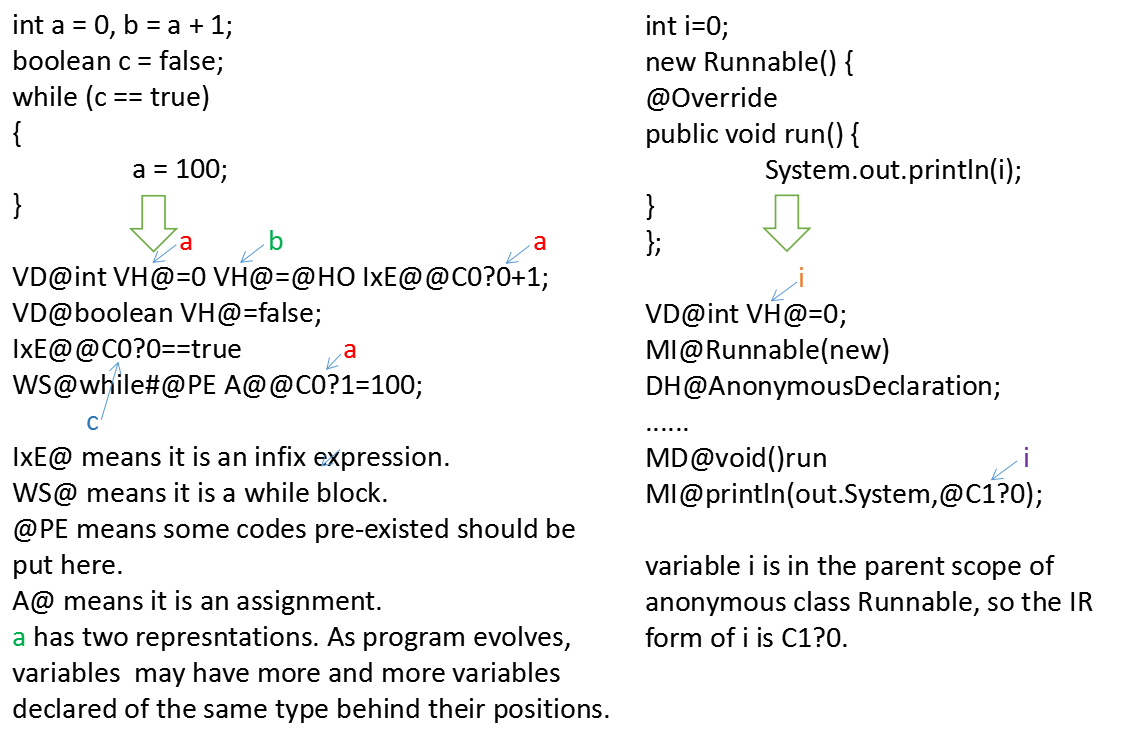
\includegraphics[width=0.48\textwidth]{pics/moreexamplesIR.png}\\
  \vspace{-0.1cm}
  \caption{More examples to IR}\label{moretoIR}
\end{figure}

In order to preserve the information as much as possible, the 8-gram model is trained.
%In order to do the genetic algorithm, the models of 1 to 7 grams are also trained.

After the 8-gram model been trained, it is put into Aero Spike\cite{aerospikedocs} which is a mature distributed key-value database.

When users are editing Java files in eclipse and pressing the shortcut keys to invoke the content assistance, the PCC code completion plugin will extract the context of the currently edited Java file, use the program processor to parse the context to IR, put the IR to the Fuzzy Matcher. The possible sequences returned by Fuzzy Matcher will be put into multiple Synthesizers to generate the final completions.

Every synthesizer runs in a separated thread. The Collector will collect all the results of all threads and append the results to the GUI of the eclipse.

\vspace{-0.1cm}
\section{N-gram Model}

The training process computes and stores all the conditional probabilities:

$P(s_m|s_{m-1}...s_{m-(n-1)}) = \frac{c(s_m...s_{m-(n-1)})}{c(s_{m-1}...s_{m-(n-1)})}$
\\where c($\cdot$) is the count of the given sequence of tokens, $s_i$ represents the token, $m \in \mathbb{Z}$ .

After training, given a sequence of tokens $s_1...s_{n-1}$ and an available n-gram model, the probability of next token is:

$NP(s_{next}) = P(s_{next}|s_1...s_{n-1}) * F(s_1...s_{n-1})$

$F(s_1...s_{n-1}) = \prod_{m=1}^{n-1}P(s_m|s_{m-1}...s_{m-(n-1)})$

\section{Fuzzy Matcher}

In most cases, The codes mined are not exactly same as the codes written by users. The fuzzy matching algorithm is combined with the genetic algorithm \cite{geneticalgorithm} and the longest common subsequence LCS algorithm \cite{introalgorithm}.

Figure \ref{fuzzymatch} gives a concrete idea about how this algorithm is running. For the sake of simplicity, the complex IR tokens are replaced by the English alphabets.
\begin{figure}[htbp]
  \centering
  % Requires \usepackage{graphicx}
  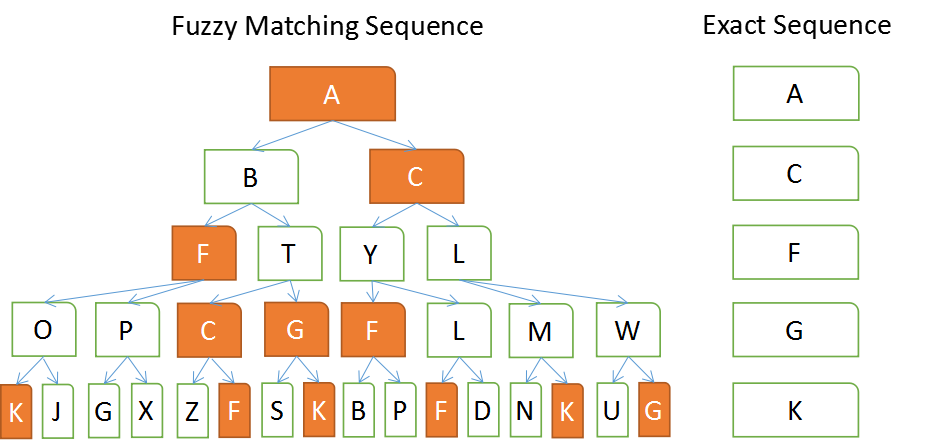
\includegraphics[width=0.42\textwidth]{pics/fuzzymatchshow.png}\\
  \caption{Fuzzy Matching Algorithm}\label{fuzzymatch}
\end{figure}
\vspace{-0.25cm}

Assume that the already written codes are A, C, F, G, and K. The fuzzy algorithm starts at A, infers the next generation of A based on 2-gram model, chooses two tokens with the highest probabilities computed by $P(token|A)$. Assume that the values of P(B|A) and P(C|A) are largest. So B and C are inferred. The longest common subsequences between the two newly generated sequences: AB, AC and the already written codes: ACFGK are computed. Then, the fuzzy algorithm does the similar things to each token of the new generation: B, C, but this time, 3-gram model is used because the length of the context is 2. Assume that the values of $P(F|AB), P(T|AB), P(Y|AC)$ and $P(L|AC)$ are largest, so, in the next generation, F, T, Y, and L are inferred. The corresponding longest common sequences are recalculated. Keep doing the algorithm until the length of the newly generated sequence is more than the length of the already written codes. In realization, 4 to 8 tokens will be inferred from a single sequence instead of 2. Through the selection of the most likely next generation, the overall search space has been reduced.

The most similar sequences will be retained which are the sequences with orange nodes on its path in Figure \ref{fuzzymatch}.
%In a lot of projects in the same field, codes are similar but not exactly same.

\section{Precise Synthesizer}

PCC puts every sequence returned by the Fuzzy Matcher to an unique Precise Synthesizer. Based on the given sequence, the Precise Synthesizer keeps using the 8-gram model to infer and synthesize the next token until the the sequence of tokens can form a statement.

%The function $InferTokens$ is used to infer the next tokens from the given sequence.

Algorithm \ref{algorsyn} shows the framework of the synthesizer. The function $SynthesizeCode$ is a recursive function which is based on depth-first search. $SynthesizeCode$ has a parameter which represents the current sequence of tokens. The function $FindBound$ finds the tokens which are a whole. For example, given the IR tokens: $mi()\quad @PE\&\&C0?0$, the bound of token: $@PE\&\&C0?0$ is $mi()$ because $mi()\&\&C0?0$ is a whole. The function $Synthesize$ keeps merging the last two tokens from the second argument back to the first argument, and involves the type checking to ensure that there are no compilation errors. If the first argument is null, the tokens from the newly inferred token back to the start of the sequence will all be merged. Figure \ref{synthesizerexample} gives a concrete idea about synthesizing one sequence.

The internal code completion in eclipse could infer the specifications based on literals. This functionality is integrated into PCC. For example, the internal code completion could translate $String$ to $java.lang.String$ or translate $a.subStr$ to $a.substring(int\ beginIndex)$.

 Because the symbol of the variable name such as $C0?0$, $F0?1$ does not contain the information about which type this symbol represents. Therefore, all the types must be tried to synthesize the code. For example, assume two variables declared: $int\ a = 0;boolean\ b = false;$, when synthesizing the code: $C0?0$<1, a<1 and b<1 are tried and b<1 is eliminated due to the type conflict.
\vspace{-0.5cm}
\\\begin {algorithm}
\caption {$SynthesizeCode(contextsequence)$}
\label{algorsyn}
\begin {algorithmic}
\REQUIRE $contextsequence != null$
\STATE $nextgenerations\leftarrow InferTokens(contextsequence)$
\FOR { $token : nextgenerations$ }
\STATE $boundtoken\leftarrow FindBound(token)$
\STATE $success\leftarrow Synthesize(boundtoken, token)$
\IF { $!success$ }
\STATE $return$
\ENDIF
\IF { $CanFormStatement(contextsequence + token)$ }
\STATE $AppendResult(Synthesize(null, token))$
\STATE $return$
\ENDIF
\STATE $SynthesizeCode(contextsequence + token)$
\ENDFOR
\end {algorithmic}
\end {algorithm}
\vspace{-0.25cm}
\\\begin{figure}
  \centering
  % Requires \usepackage{graphicx}
  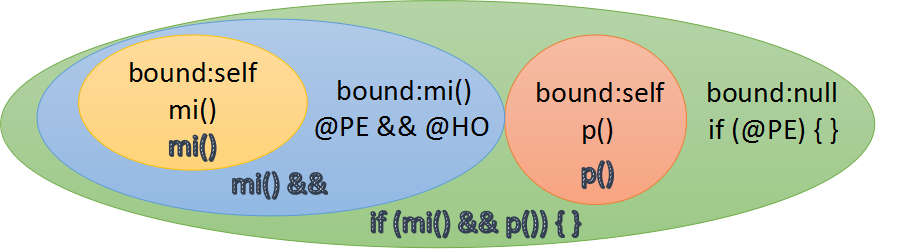
\includegraphics[width=0.4\textwidth]{pics/synthesizeexample.png}\\
  \caption{One Sequence Synthesis Example}\label{synthesizerexample}
\end{figure}
\vspace{-0.4cm}

\section{Implementation}

The source of PCC is in \cite{pccsource}. PCC is implemented in Java. PCC has 28555 lines of code. The Antlr4 \cite{antlr4} library is used to parse the special IR. The model is stored in memory. The AeroSpike database is configured to use memory as the storage device. The AeroSpike database is installed on a Linux machine. The eclipse with PCC installed is running on a Windows machine. The computers used in experiments all have 16G memory and a 2-core i7 CPU.

\section{Preparation of PCC}

Before using PCC, an AeroSpike database which is properly configured must be available.

The program of translating Java to the IR is in \cite{programprocessor}. The tutorial is in \cite{programprocessortutorial}. The bash script of training the IR to the 8-gram model is in \cite{ngramtrain}. The tutorial is in \cite{ngramtraintutorial}. The program of putting the 8-gram model into the Aero Spike database is in \cite{modeltoaero}. The corresponding tutorial is in \cite{modeltoaerotutorial}. A crawler which can crawl projects from github is in \cite{gitcrawler}. The format of the files to be downloaded is zip. A script to unzip these zipped files is available in \cite{unzipscript}.

\section{Use of PCC}

The installation way \cite{eclipseplugininstall} of the PCC tool is the same as the common plug-in \cite{eclipseplugins} of eclipse \cite{eclipseplatform}. When the AeroSpike databases filled with the 8-gram model are available, users need to set the IP address of one machine of the AeroSpike clusters on the preference page of their own eclipse. Figure \ref{GUIpreference} shows the GUI of the preference page.

When everything is ready, the only thing to do is to press the hot key of content assistance of eclipse which is usually $Alt+/$ to invoke the internal content assistance plugin and the PCC. Figure \ref{codecomprunexample} shows the screenshots of the running eclipse with the PCC installed. The proposals prefixed by the apple icon are generated by PCC. The lower the position, the higher the priority.
\vspace{-0.2cm}
\\\begin{figure}[htbp]
  \centering
  % Requires \usepackage{graphicx}
  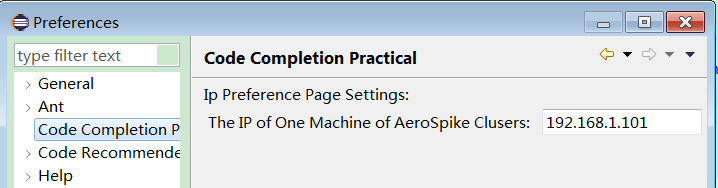
\includegraphics[width=0.48\textwidth]{pics/preferencesetting.png}\\
  \caption{GUI of IP preference setting}\label{GUIpreference}
\end{figure}
\vspace{-0.5cm}
\\\begin{figure}[htbp]
  \centering
  % Requires \usepackage{graphicx}
  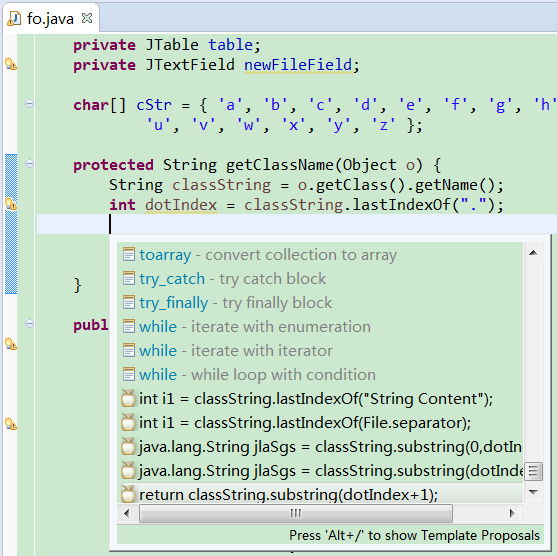
\includegraphics[width=0.42\textwidth]{pics/codecomprunexample.png}\\
  \caption{Running Screen Shot}\label{codecomprunexample}
\end{figure}
\vspace{-0.1cm}

\section{Empirical Results}

By learning different projects from github, we found that if two projects deal with different areas, only a small part is similar. Therefore, to simplify our experiments, we only choose projects which deal with similar areas.

Due to the strong type checking of PCC, the project must import the necessary jar packages, otherwise wrong codes may be obtained. In order to reduce the workload of configuring the jar packages, we choose the projects that do not require or require little external jar packages.

After screening by the two conditions just mentioned, 2187 Java files are selected to do the experiments. Due the small size of the model, we put the model into memory.

If the last five proposals returned by PCC contain the right answer, we think the completion is right.

% what is case?
We choose 10 different functions including lambda expressions in Java8. For each function, we randomly choose 10 positions. At each selected position, we invoke the content assistance. We compare the proposals returned by PPC with the actual statement following the position where we invoked the content assistance. The 100 test cases consist of these 100 positions.

The experiments show that the accuracy is 98\%. Only two test cases are not passed. One failed test case is due to too many possible choices when inferring from 7-gram. Another is due to the failure of choosing the right variable from three variables which all pass the type checks.

% how to do fuzzy testing?
In order to evaluate the performance of the fuzzy matching algorithm, we randomly add and delete one or two statements of the context of the 100 test cases, and compare the proposals returned by PPC with the actual statement.

The experiments show that the accuracy is greater than or equal to 95\%. If we randomly add some statements to the context of the 100 test cases, there is no influence on the accuracy. However, if we randomly delete some statements of the context of the 100 test cases, the accuracy decrease to 95\%. The reason for the decline in the correct rate is that the genetic algorithm fails to infer some vital tokens in the process of producing the next generation.

\section{Limitation and Future Work}

PCC automatically writes the codes if the completion context is similar to some codes in the database. The computation of the similarity is mainly based on comparing the string contents of each token. If two programs are similar in logic but not similar in structure, PCC will take them as two different programs. What is more, if two programs are structurally similar, but their method names are totally different, PCC will not generate the right code either. When the model becomes more and more large, the genetic algorithm may fail to infer some vital tokens, which leads to the bad results. The future work will mainly focus on solving the problems just mentioned.

\section{Conclusions}

We present PCC, a plugin of eclipse IDE, to automatically complete the code when users are writing Java codes in eclipse.
PCC does not influence the existing functionality of eclipse.

We make a careful analysis of the advantages and disadvantages of the existing work, put forward an IR in which one token represents one operation. Different name conventions of variables are translated into an unified form.

The fuzzy matching algorithm is applied to cope with possible changes in codes. The synthesizer involves runtime type-checking to ensure there is no compilation errors except some unresolved method invocations.

PCC is a real-time tool with quick responses. It is suitable to train some targeted sets according to different users and different projects. Users may find that many codes do not need to be written by themselves.

\newpage
%
% The following two commands are all you need in the
% initial runs of your .tex file to
% produce the bibliography for the citations in your paper.
\bibliographystyle{abbrv}
\bibliography{sigproc}  % sigproc.bib is the name of the Bibliography in this case
\end{document}
